\chapter{Subfitness}

\section{The $T_1$-axiom}

\begin{framed}
  \begin{df}[$T_1$]
    A topological space $(X, \tau)$ is said to be a \emph{$T_1$-space\/} (or to
    satisfy the \emph{$T_1$-axiom\/}) if the following holds:
    \begin{center} \it
      for any $x \ne y$ from $X$ there exists an open set $U\in \tau$ such that
      $x\in U \not\owns y$.
    \end{center}
  \end{df}
\end{framed}

\begin{figure}[h]
  \centering
  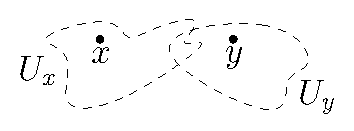
\includegraphics[height=13mm]{../img/t1.eps}
  \caption[$T_1$ property]{$T_1$ property\\
    ($U_x, U_y$ are not necessarily disjoint)}
\end{figure}

The following is a standard and useful characterization of this property.

\begin{fact} \label{T1Char}
  A topological space $X$ is $T_1$ iff $\overline{\left\{x\right\}} =
  \left\{x\right\}$ for any $x\in X$.
\end{fact}

(Of course:
if $y\not\in \left\{x\right\}$, we obtain an open $U$ such that $y\in
U\not\owns x$ and thus $y\not\in \overline{\left\{x\right\}}$.
Conversely, with open $U:= X\setminus \left\{y\right\}$ we can easily check
$(T_1)$.)

\begin{cor}
  A space is $T_1$ iff every of its finite subsets is closed.
\end{cor}

There are exact counterparts of this axiom in the point-free context (see,
e.~g.,~\cite{ds72}).
They have not found much use so far, though.
Instead, one introduces a weaker and very useful condition: {\sl the
subfitness\/}.

\section{Subfit locales}

\begin{framed}
  \begin{df}[Sfit]
    A locale $L$ is said to be \emph{subfit\/} if
    \[
      a \not\le b \qquad \Rightarrow \qquad \exists c, \quad a \vee c = 1 \ne b
      \vee c.
    \]
  \end{df}
\end{framed}

\begin{thm} \label{T1->Sfit}
  Every $T_1$-space is subfit.
\end{thm}

\begin{proof}
  For each $T_1$-space $X$ the corresponding locale $\Omega(X)$ is subfit.
  Indeed: for open $A\not\subseteq B$ there exists an $x\in A \setminus B$.
  By Fact~\ref{T1Char} we have an open $X\setminus \left\{x\right\}$.
  Since $x\in A$ and $x\not\in B$, we conclude with $A\cup (X\setminus
  \left\{x\right\}) = X \ne B \cup (X\setminus \left\{x\right\})$.
\end{proof}

The subfit topological spaces are characterized by

\begin{prop}[Isbell, Simmons] \label{Sfit-char}
  For a topological space $X$ the locale $\Omega(X)$ is subfit iff
  \[
    \forall U\in\Omega(X) \forall x\in U \exists y\in \overline{\{x\}}: \quad
    \overline{\{y\}} \subseteq U
  \]
\end{prop}
\begin{proof}
  $\Rightarrow$:
  Choose an~$x \in U$.
  Thus, we have $U\not\subseteq X\setminus \overline{\{x\}}$ and by subfitness
  an~open $V$ with $U \cup V = X \ne (X\setminus \overline{\{x\}}) \cup V$.
  Then there exists an~element $y\not\in V$ with $y\not\in X\setminus
  \overline{\{x\}}$, in other words, $y\in \overline{\{x\}}$.
  Furthermore, $V \cap \overline{\{y\}} = \none$ (for $z \in V \not\owns y$
  means $z\not\in \overline{\{y\}}$), and as $U \cup V = X$, we finish with
  $\overline{\{y\}} \subseteq U$.

  $\Leftarrow$:
  Suppose $U\not\subseteq V$ and take $x\in U\setminus V$.
  For the similar reason as above $V \cap \overline{\{x\}} = \none$.
  Let us have $y$ from the premise:
  $y \in \overline{\{x\}}$ implies  $y\not\in V$, thus, leading to $(X\setminus
  \overline{\{y\}}) \cup V \ne X$;
  and since $\overline{\{y\}} \subseteq U$ then also $(X\setminus
  \overline{\{y\}}) \cup U = X$.
\end{proof}

Here is an example of a subfit non-$T_1$-space:

\begin{exmpl}
  Let us have $X = \N \cup \left\{\infty\right\}$ and $\theta = \left\{
  F\subseteq X \st X\setminus F \Subset \N \right\} \cup \left\{ \none
  \right\}$.
  That is, $\mathcal{X} := (X, \theta)$ is the topological space where closed
  sets consist of~finite sets of~natural numbers and of~the whole space $X$.

  It is not $T_1$ for the one-point set $\left\{ \infty \right\}$ is not
  closed (see Fact~\ref{T1Char}).

  On the other hand, any open set satisfies the condition from
  Proposition~\ref{Sfit-char}:
  the empty set trivially;
  since a finite $\{x\}$ for $x\in \N$ is closed itself, we are allowed to
  put $y := x$;
  and if $x = \infty$ then $\overline{\{ \infty \}} = X$, hence we can choose
  any $y \ne \infty$ from $U$.
\end{exmpl}
